%%===========================================================%%
%%                                                           %%
%%                       INTRODUCTION                        %%
%%                                                           %%
%%===========================================================%%


\chapter{Introduction}\label{chap:introduction}

% - -- --- ---- ----- ------ ------- S E C T I O N ------- ------ ----- ---- --- -- -
\section{Central Exclusive Production}
The Central Exclusive Production (CEP) takes place when interacting particles form in the mid-rapidity region a state (``central production'') whose all constituents/decay products are measured in the detector (``exclusive''). The initial state particles can either dissociate, excite or stay intact. The latter case of CEP in proton-proton collisions can be written as
\begin{equation}\label{eq:cep}%
%  p~~+~~p~~~\rightarrow~~~p~~\stackrel{\Delta\eta_{1}}{\oplus}~~X~~\stackrel{\Delta\eta_{2}}{\oplus}~~p
p~~+~~p~~~\rightarrow~~~p~~+~~X~~+~~p
\end{equation}
and depicted as in Fig.~\ref{fig:eta_phi}. Mass and rapidity of state $X$ is given by
\begin{equation}\label{eq:mass_X}
M_{X} = \sqrt{s\Big(\xi_{1}\xi_{2}\sin^{2}{(\alpha/2)}-(1-\xi_{1}-\xi_{2})\cos^{2}{(\alpha/2)}\Big)} \stackrel{\alpha=\pi}{=} \sqrt{s\xi_{1}\xi_{2}},
\end{equation}\vspace{-10pt}
\begin{equation}\label{eq:rapidity_X}
y_{X} = \frac{1}{2}\ln{\frac{\xi_{1}}{\xi_{2}}},
\end{equation}
where $\alpha$ is angle between scattered protons and $\xi=(p_{0}-p)/p_{0}$ is the fractional momentum loss of proton.

% - -- --- ---- ----- ------ ------- S E C T I O N ------- ------ ----- ---- --- -- -
\section{Double \Pomeron\  Exchange}
Reaction from Eq.~\ref{eq:cep} can exhibit purely electromagnetic ($\gamma$-$\gamma$), mixed ($\gamma$-$\mathcal{O}$) or purely strong nature ($\mathcal{O}$-$\mathcal{O}$). The last type is dominant at RHIC energies. It is characterized by the lack of hard scale (if protons are scattered at small angles), therefore perturbative QCD cannot be applied and Regge theory~\cite{IntroductionToRegge} is used instead. An object $\mathcal{O}$ does not have direct QCD representation - in Regge framework it is the so-called ``trajectory`` (\Reg eggeon, \Reg). \Reg eggeon with quantum numbers of vacuum is called ''\Pomeron`` (\Pom) and \Pom-\Pom\ reaction (Fig.~\ref{fig:DPE}) is called ''Double \Pomeron\  Exchange``. %

%---------------------------
\begin{figure}[b!]
\centering
\parbox{0.475\textwidth}{%
  \centering%
  \hspace*{-10pt}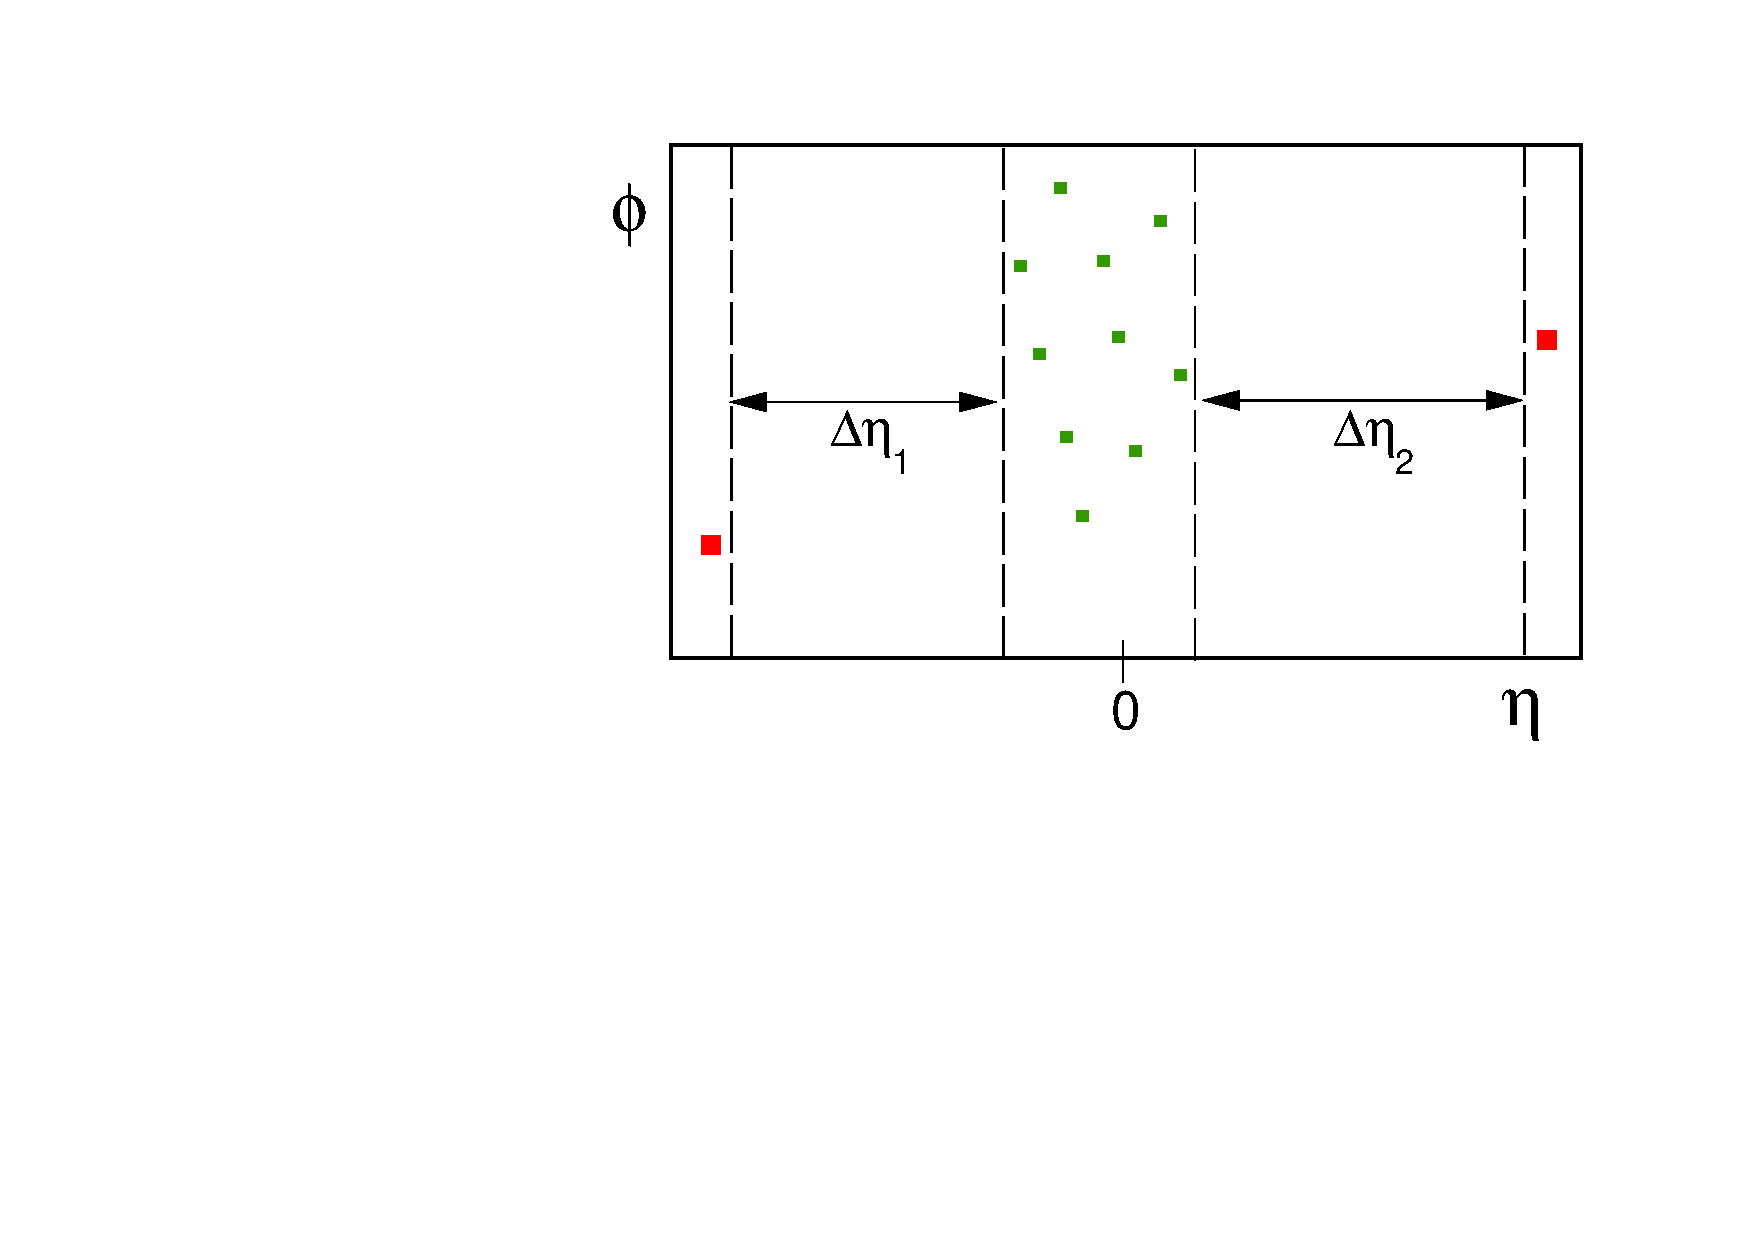
\includegraphics[width=1.1\linewidth]{graphics/introduction/eta_phi.pdf}\vspace*{-10pt}%
  \caption{Central Exclusive Production in $\eta$-$\phi$ space.\\}%
  \label{fig:eta_phi}%
}
\quad
\parbox{0.475\textwidth}{%
  \centering%
  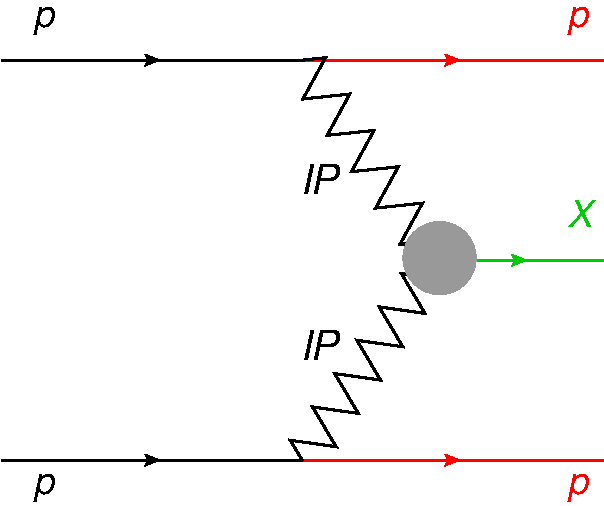
\includegraphics[width=0.64\linewidth]{graphics/introduction/DPE.pdf}%
  \caption{Diagram of D\Pom E process.\\}%
  \label{fig:DPE}%
}\vspace*{-20pt}
\end{figure}
%---------------------------

Processes involing \Pomeron\  exchange are referred as diffraction due to cross-section in scattering angle resembling similar shape to instesity pattern of diffracted light. Diffractive events have specific property of the ''rapidity gap`` which is an angular region free of hadrons. In \DPE\ two such gaps are present, marked in Fig.~\ref{fig:eta_phi} as $\Delta\eta_{1}$ and $\Delta\eta_{2}$.%

\DPE\ is a spin-parity filter - from the fact that scattered particles have all quantum numbers unchanged after the interaction, central states must satisfy
\begin{equation}\label{eq:DPE_IGJPC}
 I^{G}J^{PC}=0^{+}\textrm{even}^{++}.
\end{equation}

The lowest order QCD picture of the \Pomeron\ is a pair of oppositely colored gluons. This fact makes the \DPE\ recognized as the gluon-rich environment process which should enhance production of the bound states of gluons (''glueballs``), whose existence has not yet been proven experimentally.

For detailed introduction to the topic of diffraction see \cite{pomeronAndQCD,barone}.\vspace*{-20pt}

% - -- --- ---- ----- ------ ------- S E C T I O N ------- ------ ----- ---- --- -- -
\section{Physics motivation for the measurement}
STAR collected in 2015 large dataset dedicated for the measurement of \DPE. It has great advantage of detection of the forward protons - properties of the central state can be studied with respect to observables related to exchanged \Pomeron s. A brief list of physics issues that can be covered with this study is placed below: